%!TEX root = ../master.tex
\section{The Chinese Wall Security Policy}
The first security models that emerged were mainly concerned with military, and were thus tailored to fit the needs of the military.
\mikkel{Ved vi noget om ``hvordan''/på hvilken måde de var mainly military? Og evt hvilke modeller?}
A security policy capable of representing corporate business services was needed.
For instance an analyst that must uphold the confidentiality of his clients.
This means that he cannot advise a corporation if he has insider knowledge of a competitor.
In \citet{brewer1989chinese} such a model, \emph{The Chinese Wall}, is presented.
The concept of the Chinese Wall security policy is illustrated in \cref{chinese:illu}.
To demonstrate the purpose of the model an example of its use is given in \cref{chinese:example}.

\begin{example}{Conflict classes}\label{chinese:example}
Some firm has information about several companies; two oil companies and two banks.
In \cref{chinese:illu} this is illustrated as two groups of two companies.
These groups are in the Chinese Wall security policy known as conflict of interest classes.
When an analyst chooses to work with information about a company, he is not able to access information about other companies in the same conflict of interest class.

\begin{enumerate}
    \item The analyst chooses Shell from the leftmost conflict of interest class.
    Because of this a conceptual wall is placed around the other company in the same conflict of interest class as depicted in \cref{chinese:illu:choice1}.
    \item The analyst chooses Spar Nord from the remaining conflict of interest class.
    Now the wall shields the analyst from the rest of the Bank conflict of interest class as well.
    This can be seen in \cref{chinese:illu:choice2}.
\end{enumerate}
\end{example}

\begin{figure}
\centering
    \begin{subfigure}[t]{0.3\textwidth}
        \resizebox{\linewidth}{!}{\Large
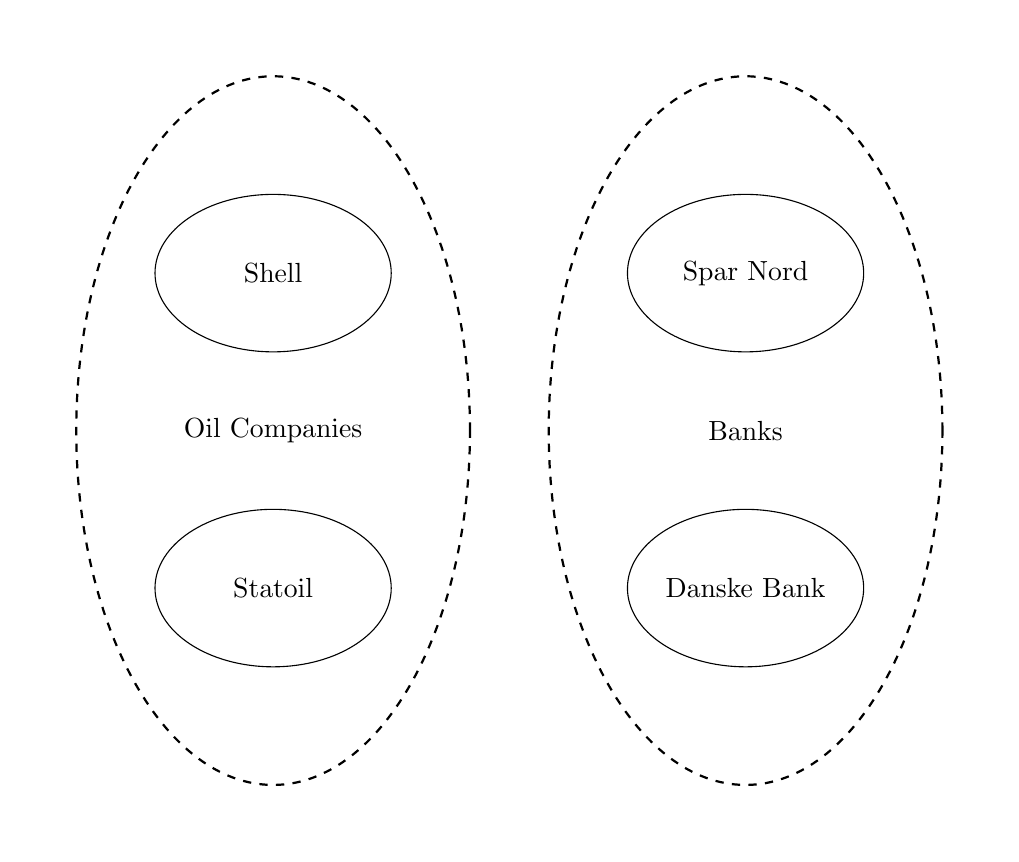
\begin{tikzpicture}
\draw  (-2,1) node{Shell} ellipse (1.5 and 1);
\draw  (4,1) node{Spar Nord} ellipse (1.5 and 1);
\draw  (-2,-3) node{Statoil} ellipse (1.5 and 1);
\draw  (4,-3) node{Danske Bank} ellipse (1.5 and 1);
\draw[thick, dashed]  (-2,-1) node{Oil Companies} ellipse (2.5 and 4.5);
\draw[thick, dashed]  (4,-1) node{Banks} ellipse (2.5 and 4.5);
\node at (1,4) {};
\node at (-5,-1) {};
\node at (7,-1) {};
\node at (1,-6) {};
\end{tikzpicture}}
        \caption{Four companies}
        \label{chinese:illu:situation}
    \end{subfigure}
    ~
    \begin{subfigure}[t]{0.3\textwidth}
        \resizebox{\linewidth}{!}{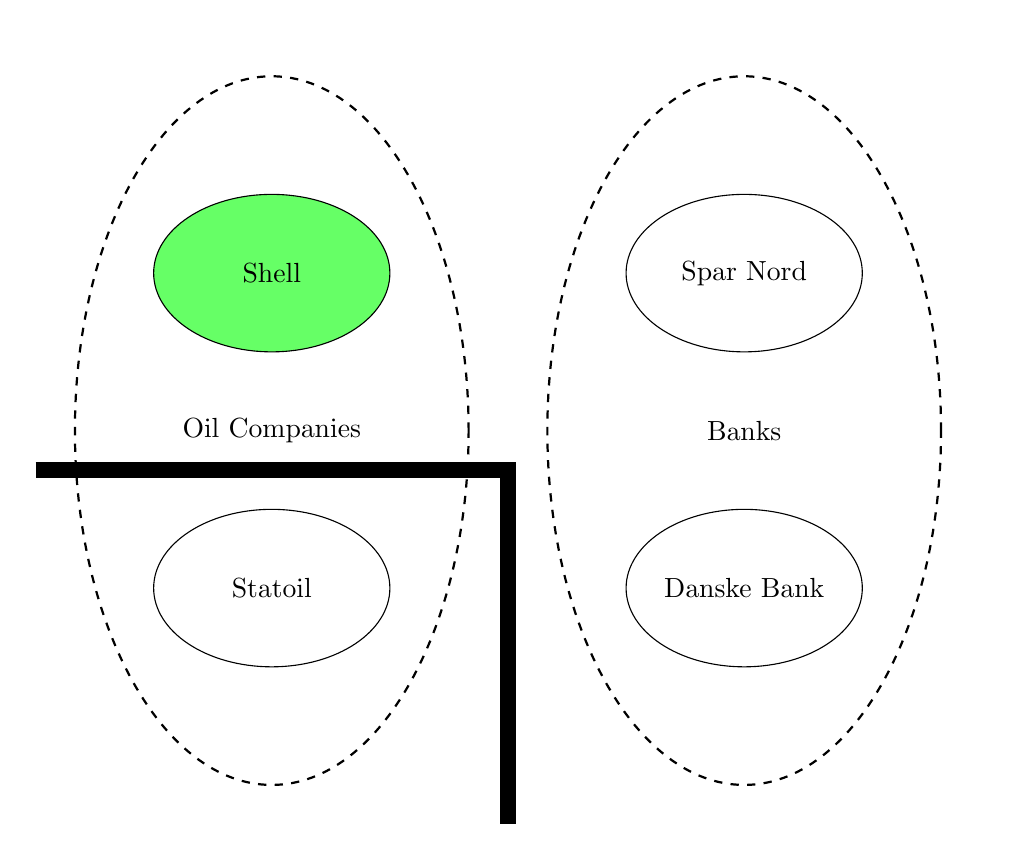
\begin{tikzpicture}

\draw[fill=green!60]  (-2,1) node{Shell} ellipse (1.5 and 1);
\draw  (4,1) node{Spar Nord} ellipse (1.5 and 1);
\draw  (-2,-3) node{Statoil} ellipse (1.5 and 1);
\draw  (4,-3) node{Danske Bank} ellipse (1.5 and 1);
\draw[thick, dashed]  (-2,-1) node{Oil Companies} ellipse (2.5 and 4.5);
\draw[thick, dashed]  (4,-1) node{Banks} ellipse (2.5 and 4.5);


\draw [line width=2mm](-5,-1.5) -- (1,-1.5) -- (1,-6);
\node at (7,0) {};
\node at (1,4) {};
\end{tikzpicture}}
        \caption{First choice}
        \label{chinese:illu:choice1}
    \end{subfigure}
    ~
    \begin{subfigure}[t]{0.3\textwidth}
        \resizebox{\linewidth}{!}{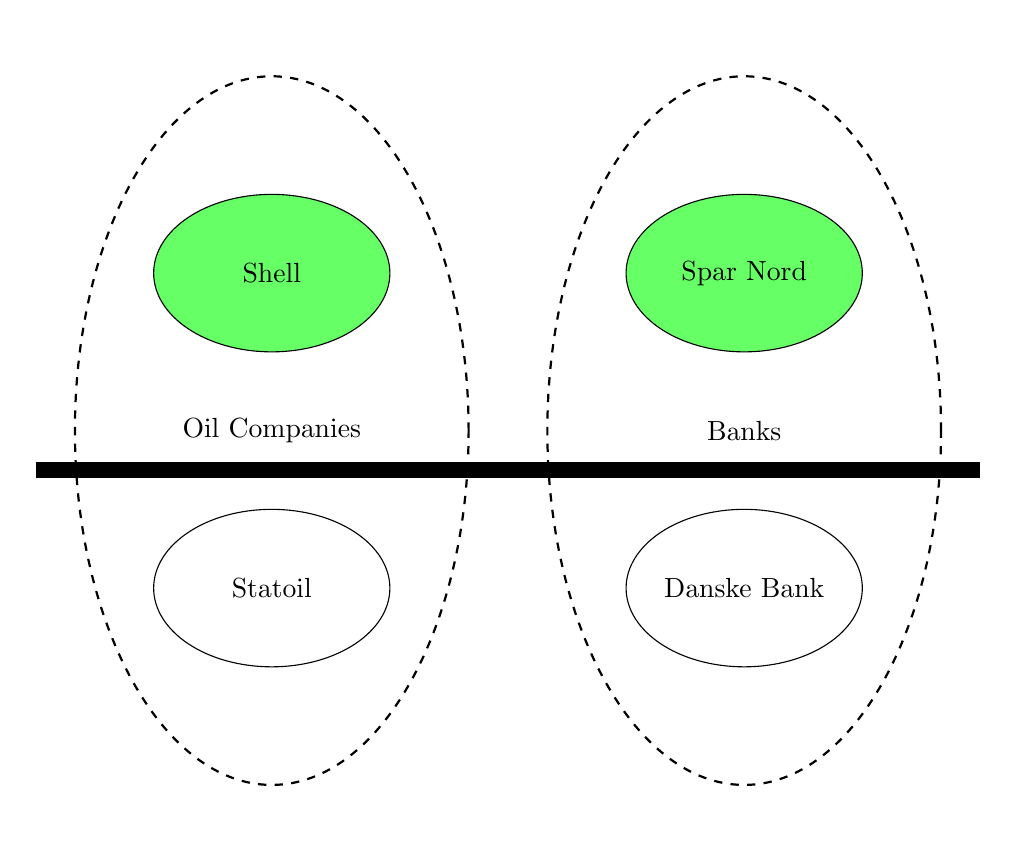
\begin{tikzpicture}

\draw[fill=green!60]  (-2,1) node{Shell} ellipse (1.5 and 1);
\draw[fill=green!60]  (4,1) node{Spar Nord} ellipse (1.5 and 1);
\draw  (-2,-3) node{Statoil} ellipse (1.5 and 1);
\draw  (4,-3) node{Danske Bank} ellipse (1.5 and 1);
\draw[thick, dashed]  (-2,-1) node{Oil Companies} ellipse (2.5 and 4.5);
\draw[thick, dashed]  (4,-1) node{Banks} ellipse (2.5 and 4.5);


\draw [line width=2mm](-5,-1.5) -- (1,-1.5) -- (7,-1.5);
\node at (1,-6) {};
\node at (1,4) {};
\end{tikzpicture}}
        \caption{Second choice}
        \label{chinese:illu:choice2}
    \end{subfigure}
    \caption{The Chinese Wall security policy}\label{chinese:illu}
\end{figure}


\subsection*{The Chinese Wall Model}
As exemplified in \cref{chinese:example} a Chinese wall is defined as the separation between what can be accessed and what cannot be accessed by the a user of the system.
Information is stored in a hierarchy with three levels. 
This hierarchy is depicted in \cref{china:hierarchy}.

\begin{itemize}
	\item The lowest level contains individual items of information, stored in objects.
	\item The middle level contains company datasets that group all information that concern one company. 
	\item The highest level contains conflict of interest classes which group companies that are in competition.
\end{itemize}

\begin{figure}[h]
  \resizebox{\textwidth}{!}{
	\begin{tikzpicture}


\node[fill=black,regular polygon, regular polygon sides=3,inner sep=1.5pt] (v3) at (-2,0) {};
\node[fill=black,regular polygon, regular polygon sides=3,inner sep=1.5pt] (v2) at (-3,0) {};


\node[fill=black,regular polygon, regular polygon sides=3,inner sep=1.5pt] (v4) at (-1,0) {};

\draw (v2) -- (v3) -- (v4);
\node (v7) at (-2,1) {Statoil};
\draw (v2) -- (v3) -- (v4);

\node (v14) at (0,1) {};
\node (v13) at (2,1) {Shell};
\node[fill=black, , regular polygon sides=3,inner sep=1.5pt] (v10) at (2,0) {};
\node[fill=black,regular polygon, regular polygon sides=3,inner sep=1.5pt] (v9) at (1,0) {};



\node[fill=black,regular polygon, regular polygon sides=3,inner sep=1.5pt] (v11) at (3,0) {};
\draw  (v9) -- (v10) -- (v11) ;

\node (v15) at (0,2) {Oil Companies};
\draw  (v14) edge (v15);




\node (v30) at (4,2) {};
\node (v40)at (8,2) {Banks};
\node (v23) at (8,1) {};
\node (v22) at (6,1) {Danske Bank};
\node (v24) at (10,1) {Spar Nord};
\node[fill=black,regular polygon, regular polygon sides=3,inner sep=1.5pt] (v25) at (10,0) {};
\node[fill=black,regular polygon, regular polygon sides=3,inner sep=1.5pt] (v28) at (9,0) {};



\node[fill=black,regular polygon, regular polygon sides=3,inner sep=1.5pt] (v29) at (11,0) {};
\node[fill=black,regular polygon, regular polygon sides=3,inner sep=1.5pt] (v18) at (6,0) {};
\node[fill=black,regular polygon, regular polygon sides=3,inner sep=1.5pt] (v17) at (5,0) {};



\node[fill=black,regular polygon, regular polygon sides=3,inner sep=1.5pt] (v19) at (7,0) {};
\draw (v17) -- (v18) -- (v19);

\draw (v23) -- (v40) -- (v30) -- (v15);
\node (v31) at (4,3) {Objects};
\draw  (v30) edge (v31);


\node at (-5,3) {\parbox{5cm}{The set of all objects}};
\draw[dashed, gray] (-3.8, 3) -- (v31);
\node at (-5,2) {\parbox{5cm}{Conflict of interest classes}};
\draw[dashed, gray] (-2.8, 2) -- (v15);
\node at (-5,0) {\parbox{5cm}{Individual data objects}};
\draw[dashed, gray] (-4.1, 1) -- (v7);
\node at (-5,1) {\parbox{5cm}{Company datasets}};
\draw[dashed, gray] (-3.4, 0) -- (v2);
\draw  (v3) edge (v7);
\draw  (v13) edge (v10);
\draw  (v22) edge (v18);
\draw  (v25) edge (v24);
\draw  (v7) edge (v14);
\draw  (v13) edge (v14);
\draw  (v22) edge (v23);
\draw  (v24) edge (v23);
\draw (v28) -- (v25) -- (11,0);
\end{tikzpicture}}
	\caption{The hierarchy of the Chinese Wall model.}
	\label{china:hierarchy}
\end{figure}

\subsection{The Security Policy}
The concept of the Chinese wall security policy is that a \principal{} that has access to information about company A which resides in a conflict of interest class C cannot access information about company B if B is also in conflict of interest class C.

In \cref{china:hierarchy} one conflict of interest class is \emph{Oil companies}.
This conflict class contains \emph{Statoil} and \emph{Shell}. 
\emph{Shell} contains objects of information that could compromise the company if \emph{Statoil} would obtain the information.
An analyst concerned with \emph{Shell} should not be able to read any information about \emph{Statoil} in order to uphold confidentiality, as was also described in the introduction.

\subsection{Chinese wall properties}
This policy is being upheld by two properties.
These correspond to the two identical properties defined in Bell Lapadula described in \cref{bellap:properties}.

\paragraph{Simple Security}

When a \principal{} S requests to read an object O, this can only be permitted if one of the following requirements are fulfilled:

\begin{itemize}
\item O is in the same company dataset as an object already accessed by S (the object is within the wall).
\item O belongs to a different interest class than any of those S has previously accessed.
\end{itemize}

\paragraph{*-Property}

When a \principal{} S requests to write to an object O if the following requirements are both fulfilled.

\begin{itemize}
\item Access to O is permitted by the simple security rule.
\item No objects from another object P in another company dataset D, which contains unsanitized information can be read when requesting write access to O.
\end{itemize}

The second requirements ensures that unsanitized information cannot leave the company dataset, but it is still possible to sanitize the data in order to compare companies.
\mads{\#42 Bedre forklaring af BLP *prop}